%% Copyright 2009 Ivan Griffin
%
% This work may be distributed and/or modified under the
% conditions of the LaTeX Project Public License, either version 1.3
% of this license or (at your option) any later version.
% The latest version of this license is in
%   http://www.latex-project.org/lppl.txt
% and version 1.3 or later is part of all distributions of LaTeX
% version 2005/12/01 or later.
%
% This work has the LPPL maintenance status `maintained'.
% 
% The Current Maintainer of this work is Ivan Griffin
%
% This work consists of the files tcp_state_machine.tex

%Description
%-----------
%tcp_state_machine.tex - an example file illustrating the TCP (RFC 793)
%                        state machine

%Created 2009-11-20 by Ivan Griffin.  Last updated: 2009-11-20
%-------------------------------------------------------------
\documentclass{article}

\usepackage{tikz}
\usetikzlibrary{calc,backgrounds}

\begin{document}

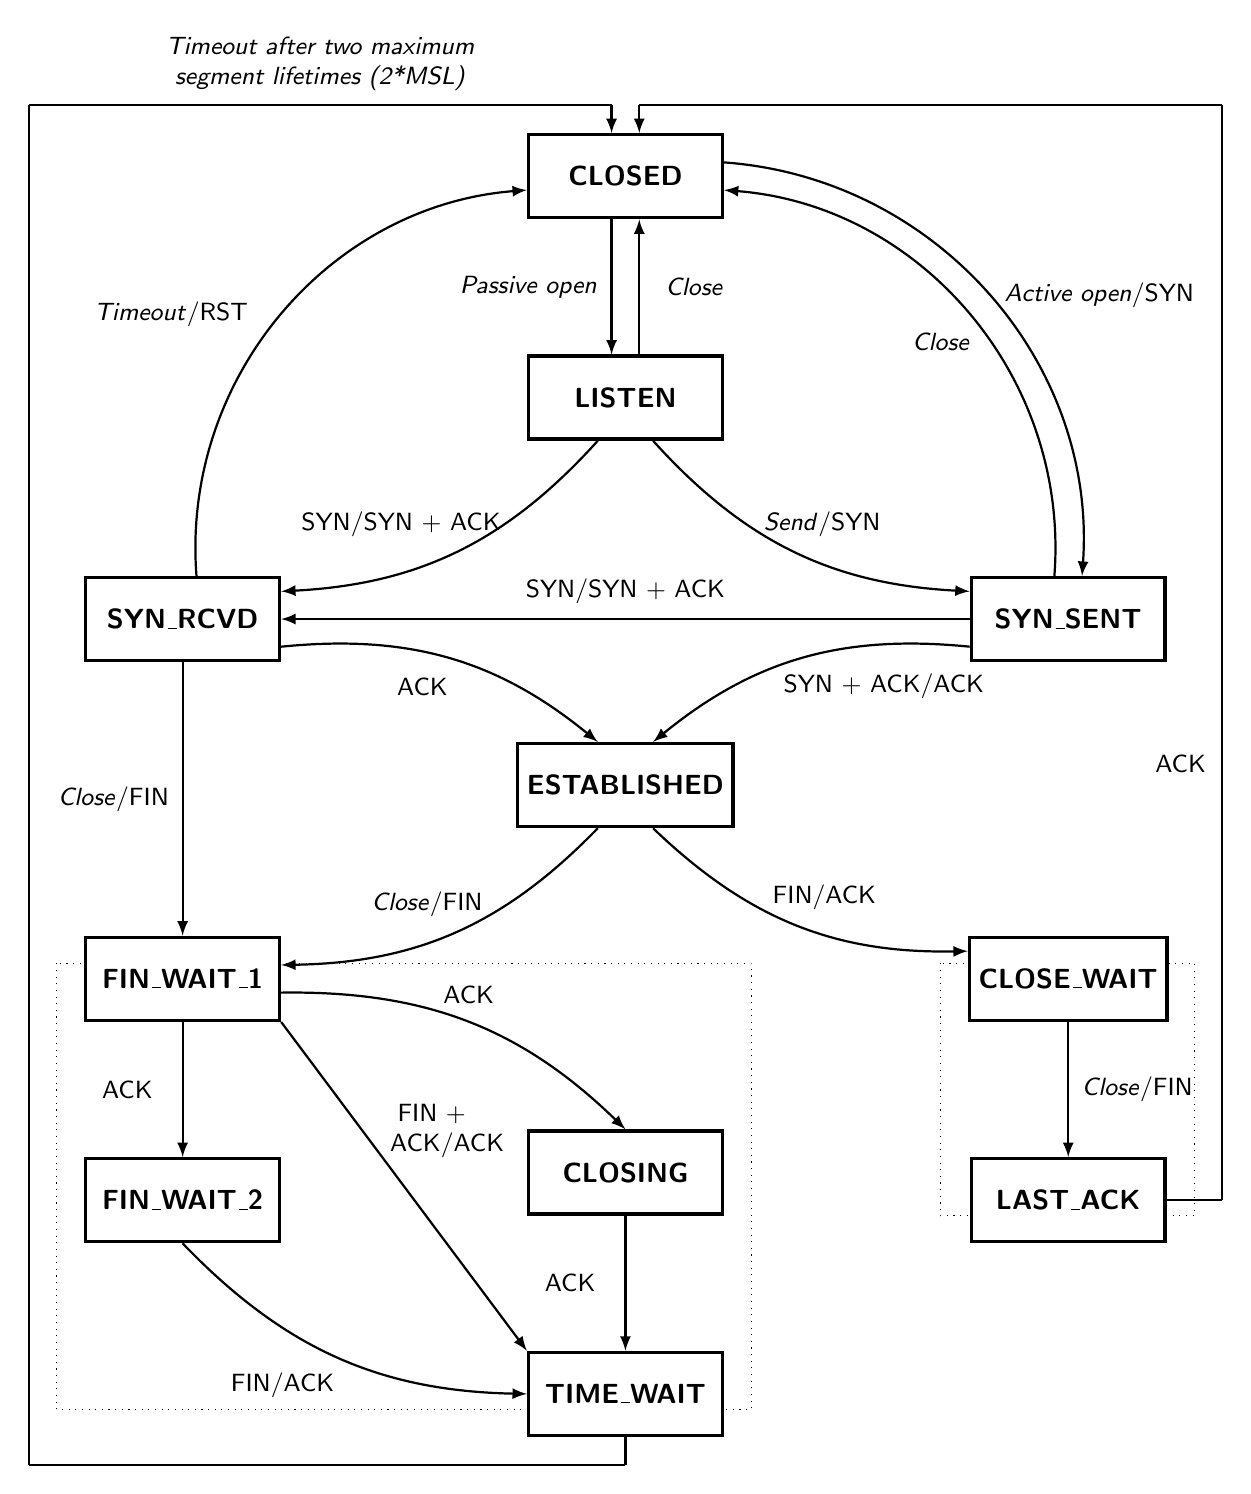
\begin{tikzpicture}[>=latex]

  %
  % Styles for states, and state edges
  %
  \tikzstyle{state} = [draw, very thick, fill=white, rectangle, minimum height=3em, minimum width=7em, node distance=8em, font={\sffamily\bfseries}]
  \tikzstyle{stateEdgePortion} = [black,thick];
  \tikzstyle{stateEdge} = [stateEdgePortion,->];
  \tikzstyle{edgeLabel} = [pos=0.5, text centered, font={\sffamily\small}];

  %
  % Position States
  %
  \node[state, name=closedStart] {CLOSED};
  \node[state, name=listen, below of=closedStart] {LISTEN};
  \node[state, name=synSent, below of=listen, right of=listen, xshift=8em] {SYN\_SENT};
  \node[state, name=synRcvd, below of=listen, left of=listen, xshift=-8em] {SYN\_RCVD};
  \node[state, name=established, below of=listen, node distance=14em] {ESTABLISHED};
  \node[state, name=finWait1, below of=established, left of=established, node distance=7em, xshift=-9em] {FIN\_WAIT\_1};
  \node[state, name=finWait2, below of=finWait1] {FIN\_WAIT\_2};
  \node[state, name=closeWait, below of=established, right of=established, node distance=7em, xshift=9em] {CLOSE\_WAIT};
  \node[state, name=closing, below of=established, node distance=14em] {CLOSING};
  \node[state, name=lastAck, below of=closeWait] {LAST\_ACK};
  \node[state, name=timeWait, below of=closing] {TIME\_WAIT};

  %
  % Connect States via edges
  %
  \draw ($(closedStart.south) + (-.5em,0)$) 
      edge[stateEdge] node[edgeLabel, xshift=-3em]{\emph{Passive open}} 
      ($(listen.north) + (-.5em,0)$); 
  \draw ($(listen.north) + (.5em,0)$) 
      edge[stateEdge] node[edgeLabel, xshift=2em]{\emph{Close}} 
      ($(closedStart.south) + (.5em,0)$);

  \draw ($(listen.south) + (-1em,0)$) 
      edge[stateEdge, bend left=22.5] node[edgeLabel, xshift=-2em, yshift=1em]{SYN/SYN + ACK} 
      ($(synRcvd.east) + (0,1em)$);
  \draw ($(listen.south) + (1em,0)$) 
      edge[stateEdge, bend right=22.5] node[edgeLabel, xshift=1em, yshift=1em]{\emph{Send}/SYN} 
      ($(synSent.west) + (0,1em)$);

  \draw ($(synRcvd.north) + (.5em,0)$) 
      edge[stateEdge, bend left=45] node[edgeLabel,xshift=-4em]{\emph{Timeout}/RST} 
      ($(closedStart.west) + (0,-.5em)$);

  \draw ($(synSent.north) + (-.5em,0)$) 
      edge[stateEdge, bend right=45] node[edgeLabel,xshift=-1em, yshift=-1em]{\emph{Close}} 
      ($(closedStart.east) + (0,-.5em)$);
  \draw ($(closedStart.east) + (0,.5em)$) 
      edge[stateEdge, bend left=45] node[edgeLabel,xshift=4em]{\emph{Active open}/SYN} 
      ($(synSent.north) + (.5em,0)$);

  \draw (synSent.west) 
      edge[stateEdge] node[edgeLabel, yshift=1em]{SYN/SYN + ACK} 
      (synRcvd.east);
  \draw (synRcvd) 
      edge[stateEdge] node[edgeLabel, xshift=-2.5em]{\emph{Close}/FIN} 
      (finWait1);

  \draw ($(synRcvd.east) + (0,-1em)$) 
      edge[stateEdge, bend left=22.5] node[edgeLabel, xshift=-1em, yshift=-1em]{ACK} 
      ($(established.north) + (-1em,0)$);
  \draw ($(synSent.west) + (0,-1em)$) 
      edge[stateEdge, bend right=22.5] node[edgeLabel, xshift=3em, yshift=-1em]{SYN + ACK/ACK} 
      ($(established.north) + (1em,0)$);

  \draw ($(established.south) + (-1em,0)$) 
      edge[stateEdge, bend left=22.5] node[edgeLabel, xshift=-1em, yshift=1em]{\emph{Close}/FIN} 
      ($(finWait1.east) + (0,.5em)$);
  \draw ($(established.south) + (1em,0)$) 
      edge[stateEdge, bend right=22.5] node[edgeLabel, xshift=1em, yshift=1em]{FIN/ACK} 
      ($(closeWait.west) + (0,1em)$);

  \draw (finWait1.south) 
      edge[stateEdge] node[edgeLabel, xshift=-2em]{ACK} 
      (finWait2.north);
  \draw ($(finWait1.east) + (0,-.5em)$) 
      edge[stateEdge, bend left=22.5] node[edgeLabel, yshift=1em]{ACK} 
      (closing.north);
  \draw (finWait1.south east) 
      edge[stateEdge] node[edgeLabel, xshift=1em, yshift=2em, text width=3em]{FIN + ACK/ACK} 
      (timeWait.north west);

  \draw (finWait2.south) 
      edge[stateEdge, bend right=22.5] node[edgeLabel, xshift=-2em, yshift=-1em]{FIN/ACK} 
      (timeWait.west);

  \draw (closing) 
      edge[stateEdge] node[edgeLabel, xshift=-2em]{ACK} 
      (timeWait);

  \draw (closeWait) 
      edge[stateEdge] node[edgeLabel,xshift=2.5em]{\emph{Close}/FIN} 
      (lastAck);

  %
  % Connect lastAck to closed is slightly more complicated
  % no direct line-of-sight, so we need to take the scenic route
  %
  \coordinate (lastAck2ClosedA) at ($(lastAck.east) + (2em,0)$);
  \coordinate (lastAck2ClosedB) at ($(closedStart.north -| lastAck.east) + (2em,1em)$);
  \coordinate (lastAck2ClosedC) at ($(closedStart.north) + (0.5em,1em)$);
  \draw (lastAck.east) edge[stateEdgePortion] (lastAck2ClosedA);
  \draw (lastAck2ClosedA) edge[stateEdgePortion] node[edgeLabel,xshift=-1.5em, yshift=-4em]{ACK} (lastAck2ClosedB);
  \draw (lastAck2ClosedB) edge[stateEdgePortion] (lastAck2ClosedC);
  \draw (lastAck2ClosedC) edge[stateEdge] ($(closedStart.north) + (0.5em,0)$);

  %
  % likewise for timeWait to closed
  %
  \coordinate (timeWait2ClosedA) at ($(timeWait.south) + (0,-1em)$);
  \coordinate (timeWait2ClosedB) at ($(timeWait.south -| finWait2.west) + (-2em,-1em)$);
  \coordinate (timeWait2ClosedC) at ($(closedStart.north -| finWait2.west) + (-2em,1em)$);
  \coordinate (timeWait2ClosedD) at ($(closedStart.north) + (-0.5em,1em)$);
  \draw (timeWait.south) edge[stateEdgePortion] (timeWait2ClosedA);
  \draw (timeWait2ClosedA) edge[stateEdgePortion] (timeWait2ClosedB);
  \draw (timeWait2ClosedB) edge[stateEdgePortion] (timeWait2ClosedC);
  \draw (timeWait2ClosedC) edge[stateEdgePortion] 
    node[edgeLabel, text width=12.25em, yshift=1.5em]{\emph{Timeout after two maximum segment lifetimes (2*MSL)}} 
    (timeWait2ClosedD);
  \draw (timeWait2ClosedD) edge[stateEdge] ($(closedStart.north) + (-0.5em,0)$);

  % draw dotted lines around passive and active closes
  \begin{pgfonlayer}{background}
    \draw [join=round,black,dotted] ($(closeWait.north west) + (-1em, -1em)$) rectangle ($(lastAck.south east) + (1em, 1em)$);
    \draw [join=round,black,dotted] ($(finWait1.north west) + (-1em, -1em)$) rectangle ($(timeWait.south east) + (1em, 1em)$);
  \end{pgfonlayer}

\end{tikzpicture}

\end{document}
